To empirically validate the optimal preprocessing and feature extraction strategy for the lane detection pipeline, a comparative analysis was conducted across nine distinct bowling video clips. These clips were specifically selected to encompass a variety of challenging real-world conditions, including varying camera exposures, surface glare, and heterogeneous lighting. The study evaluated the combinatorial performance of five single-channel transformations (Default Grayscale, Lightness, Hue, $R+G-B$, and PCA) paired with three standard edge detection algorithms (Sobel, Canny, and Laplacian). A trial was deemed successful strictly if the resulting gradient map enabled the subsequent Hough Transform and heuristic filters to correctly segment the entire playing surface by accurately isolating all four geometric boundaries (the foul line, the pin deck, and both lateral gutters), as demonstrated in Figure \ref{fig:trial_success}. The quantitative success rates for each combination are detailed in Table \ref{tab:ablation_results}.

\begin{figure}[htbp]
    \centering
    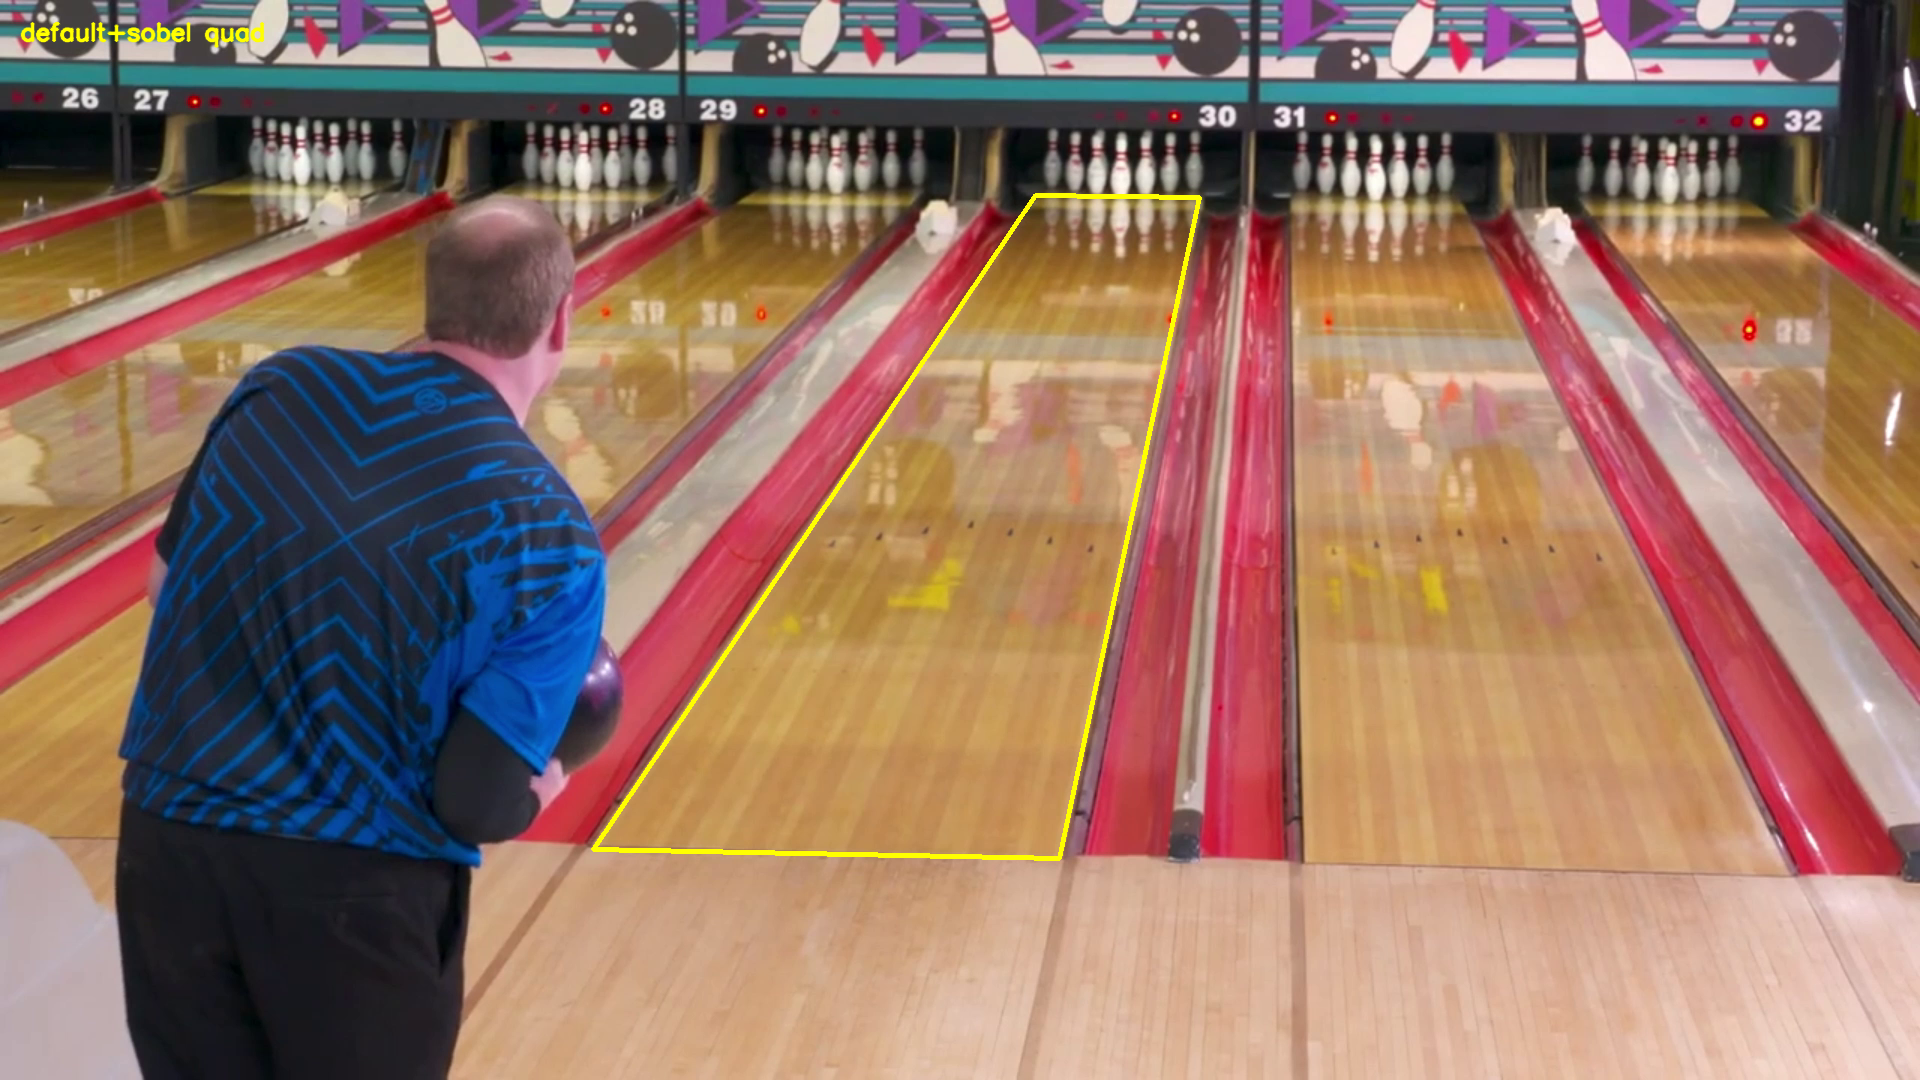
\includegraphics[width=0.48\textwidth]{figures/results/correct_lane_detection.png}
    \hfill
    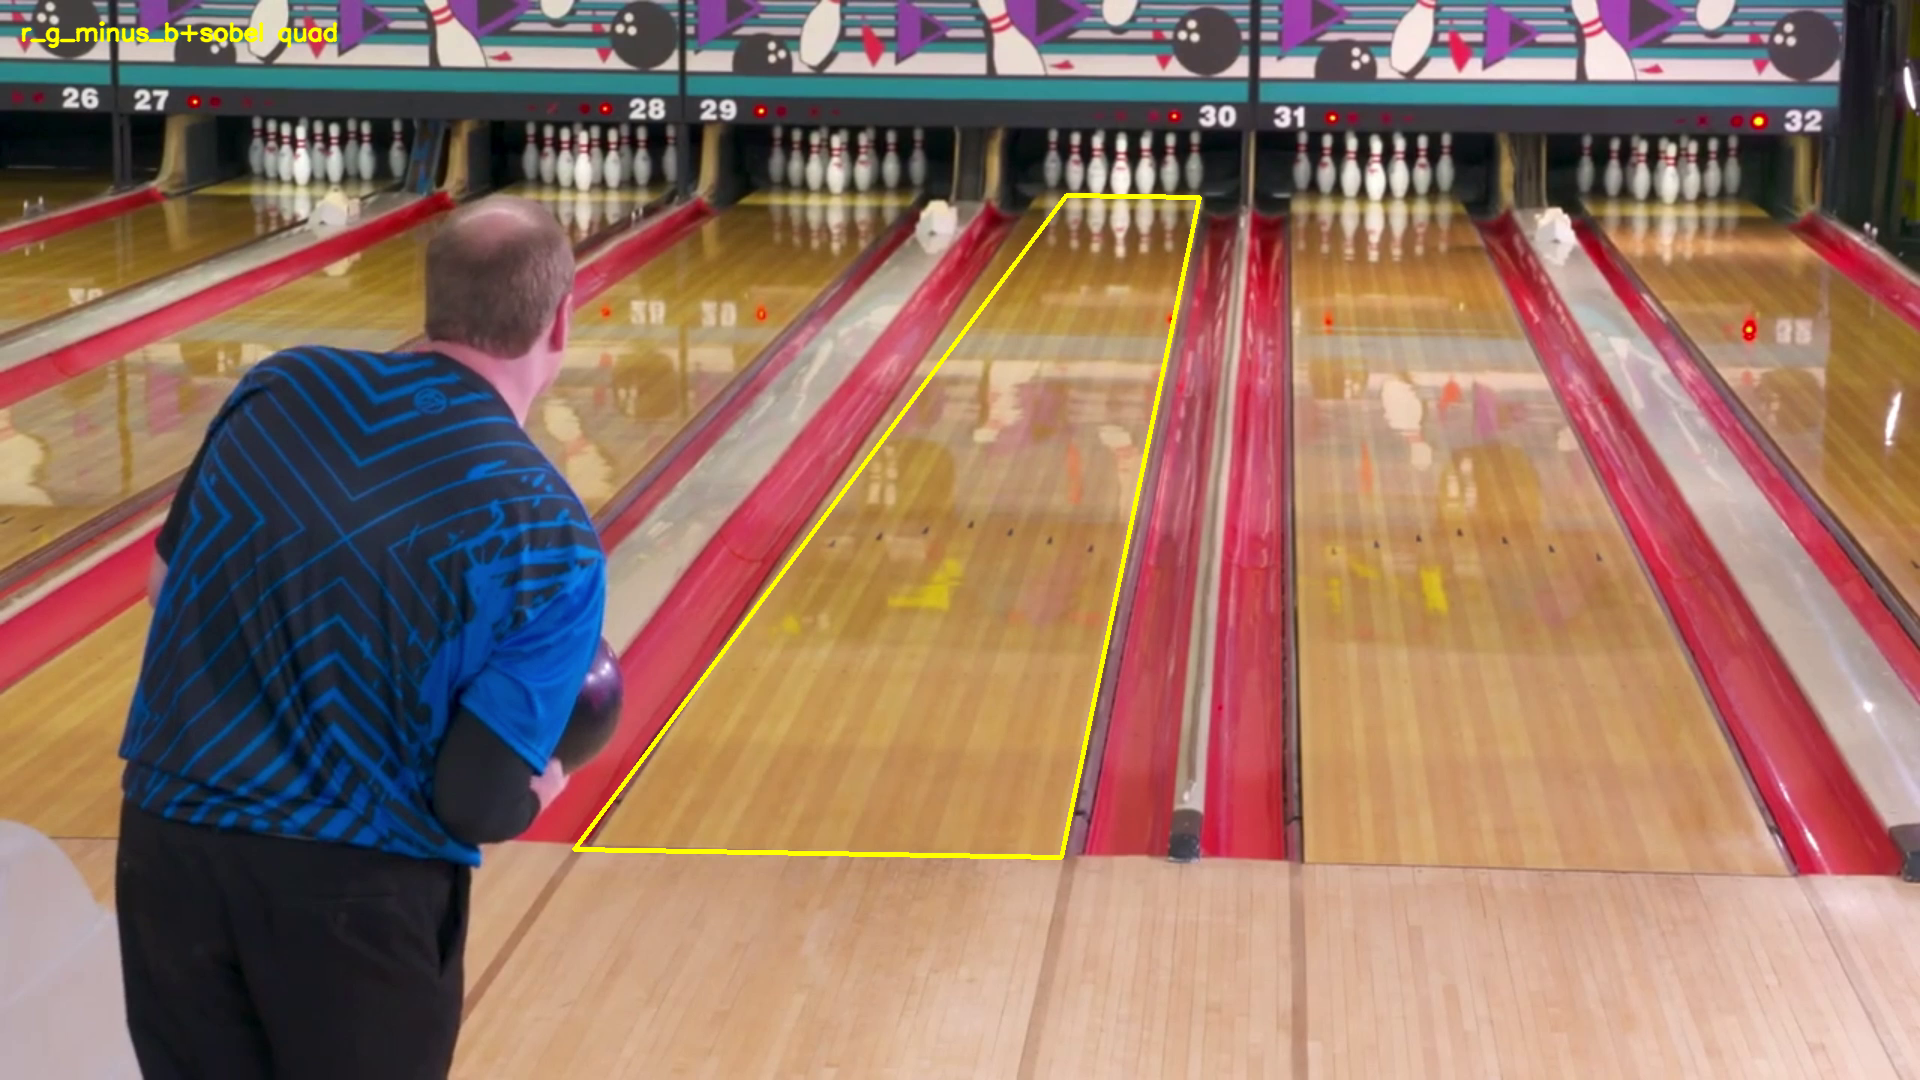
\includegraphics[width=0.48\textwidth]{figures/results/incorrect_lane_detection.png}
    \caption{Criteria for segmentation success. Left: A successful trial where the estimated quadrilateral accurately isolates the true playing surface. Right: An unsuccessful trial where the left boundary is not correctly detected.}
    \label{fig:trial_success}
\end{figure}

% --- TABLE OF RESULTS ---
\begin{table}[htbp]
\centering
\caption{Quantitative success rates of boundary detection for each preprocessing and edge detection combination across 9 video clips.}
\label{tab:ablation_results}
% This line automatically scales the table to the width of the text:
\resizebox{\textwidth}{!}{%
\begin{tabular}{llcccccccccc}
\toprule
\textbf{Grayscale Method} & \textbf{Edge Method} & \textbf{clip1} & \textbf{clip2} & \textbf{clip3} & \textbf{clip5} & \textbf{clip6} & \textbf{clip7} & \textbf{clip8} & \textbf{clip11} & \textbf{clip13} & \textbf{Sum} \\
\midrule
default & sobel & 1 & 1 & 1 & 0 & 1 & 1 & 0 & 1 & 0 & 6 \\
default & canny & 0 & 0 & 0 & 0 & 0 & 1 & 0 & 1 & 0 & 2 \\
default & laplacian & 0 & 0 & 1 & 0 & 1 & 1 & 0 & 1 & 1 & 5 \\
\midrule
lightness & sobel & 1 & 1 & 0 & 0 & 0 & 1 & 0 & 1 & 1 & 5 \\
lightness & canny & 1 & 0 & 1 & 0 & 0 & 0 & 0 & 1 & 0 & 3 \\
lightness & laplacian & 0 & 0 & 1 & 0 & 0 & 0 & 0 & 1 & 1 & 3 \\
\midrule
hue & sobel & 0 & 0 & 0 & 0 & 0 & 0 & 0 & 0 & 0 & 0 \\
hue & canny & 0 & 0 & 0 & 0 & 0 & 0 & 0 & 0 & 0 & 0 \\
hue & laplacian & 0 & 1 & 1 & 0 & 0 & 0 & 0 & 0 & 0 & 2 \\
\midrule
r\_g\_minus\_b & sobel & 1 & 0 & 0 & 1 & 1 & 1 & 0 & 0 & 0 & 4 \\
r\_g\_minus\_b & canny & 1 & 1 & 1 & 1 & 0 & 1 & 0 & 0 & 0 & 5 \\
r\_g\_minus\_b & laplacian & 1 & 1 & 1 & 0 & 0 & 0 & 0 & 0 & 0 & 3 \\
\midrule
pca & sobel & 1 & 1 & 1 & 1 & 1 & 1 & 0 & 1 & 0 & 7 \\
pca & canny & 1 & 0 & 0 & 1 & 1 & 0 & 0 & 1 & 0 & 4 \\
pca & laplacian & 0 & 0 & 1 & 0 & 1 & 1 & 0 & 1 & 1 & 5 \\
\bottomrule
\end{tabular}%
} % Closes the resizebox
\end{table}


An analysis of the aggregated results reveals clear performance disparities not only among the color transformations but, crucially, among the edge detection algorithms. The Sobel operator emerged as the generally strongest edge detection method for correctly identifying lane borders, outperforming Canny and Laplacian across the most effective grayscale transformations. While the multi-stage Canny detector and the second-order Laplacian filter are exceptionally strong edge detectors, this extreme sensitivity proved detrimental in a visually cluttered bowling alley. Qualitative analysis of the failed clips revealed that Canny and Laplacian frequently detected crisp, high-contrast edges entirely outside the target playing surface, such as architectural lines on the background wall, adjacent lane gutters, or the bowler's silhouette. These highly defined but irrelevant structures generated overwhelmingly strong candidate lines in the Hough space. Consequently, these false positives bypassed the spatial and geometric heuristics of the pipeline, leading to incorrect boundary selection and severely deformed segmentation quadrilaterals (see Figure \ref{fig:over_sensitive_edges}). Sobel, by providing a more subdued and directionally targeted gradient map, allowed the geometric filters to consistently lock onto the true lane boundaries.

% --- FIGURES ---
\begin{figure}[htbp]
    \centering
    % Top Row: The edge detection maps
    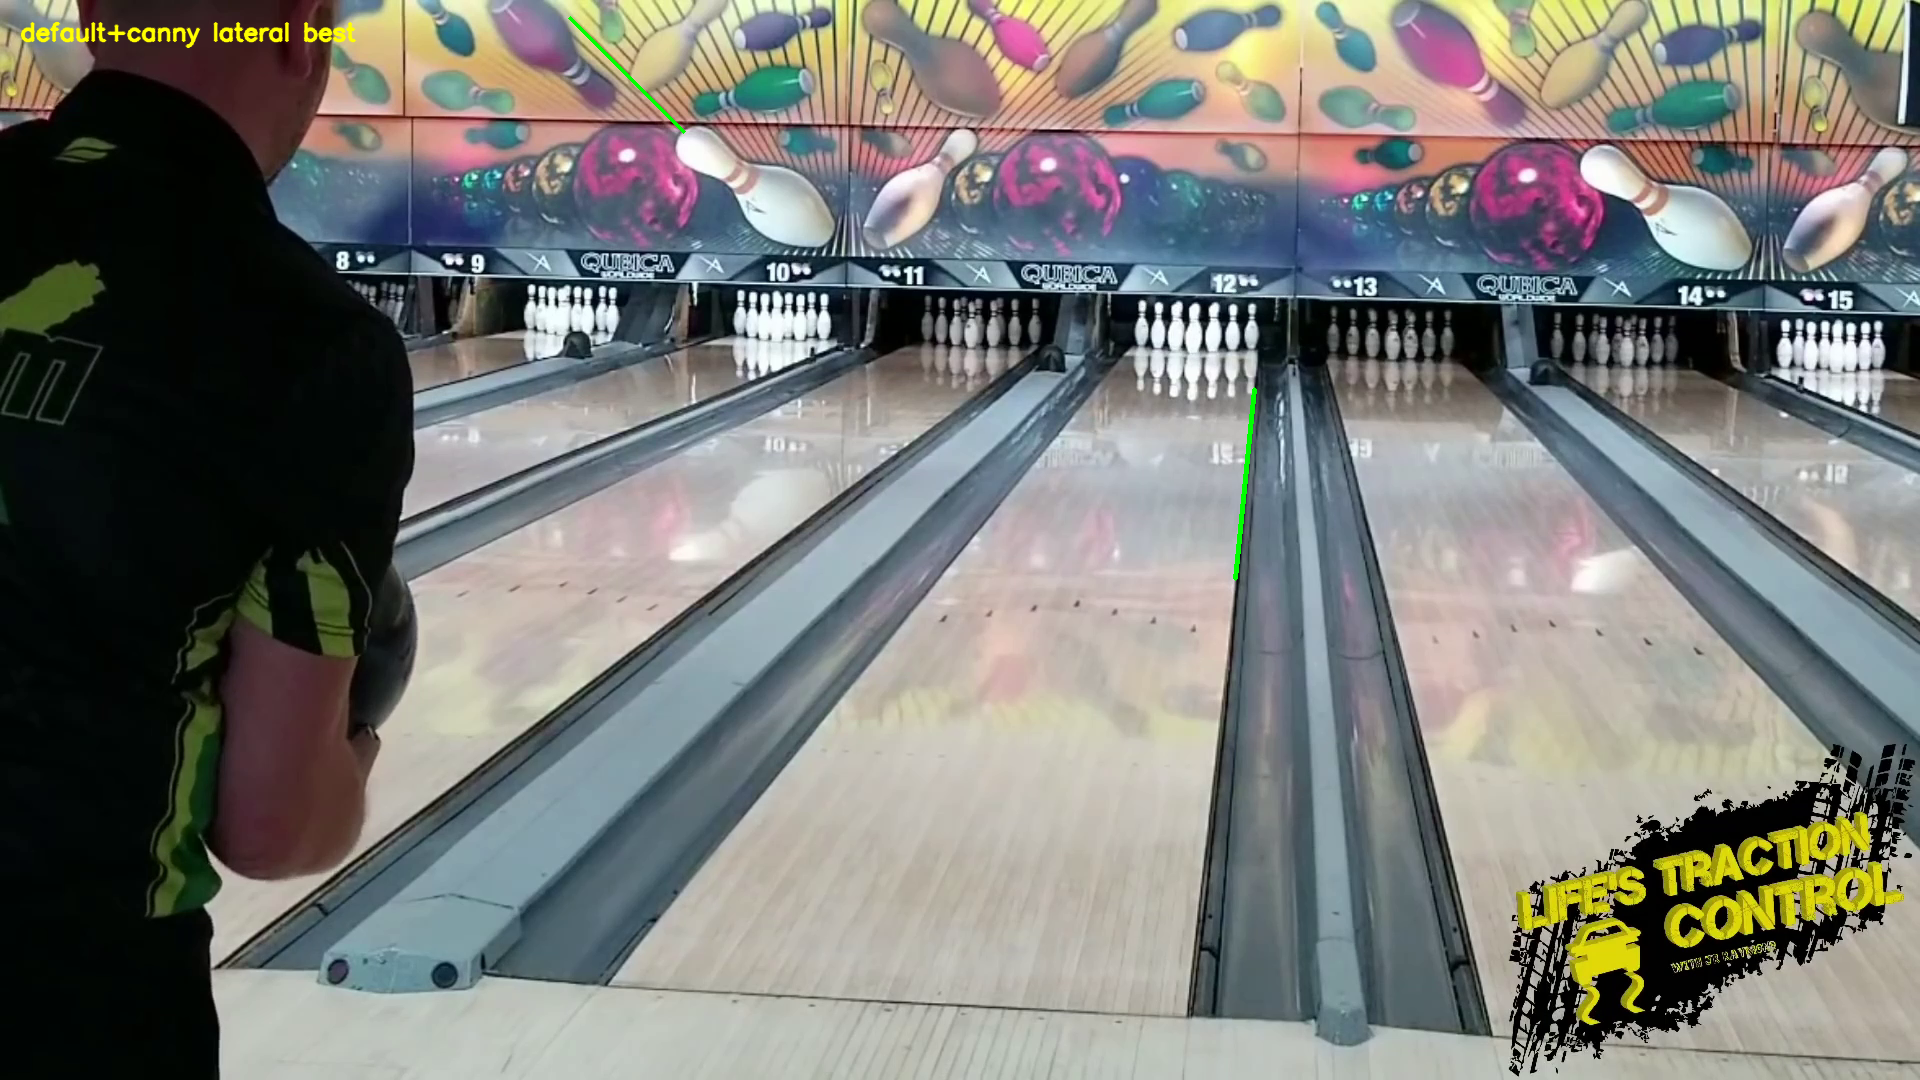
\includegraphics[width=0.48\textwidth]{figures/results/canny_over_sensitive.png}
    \hfill
    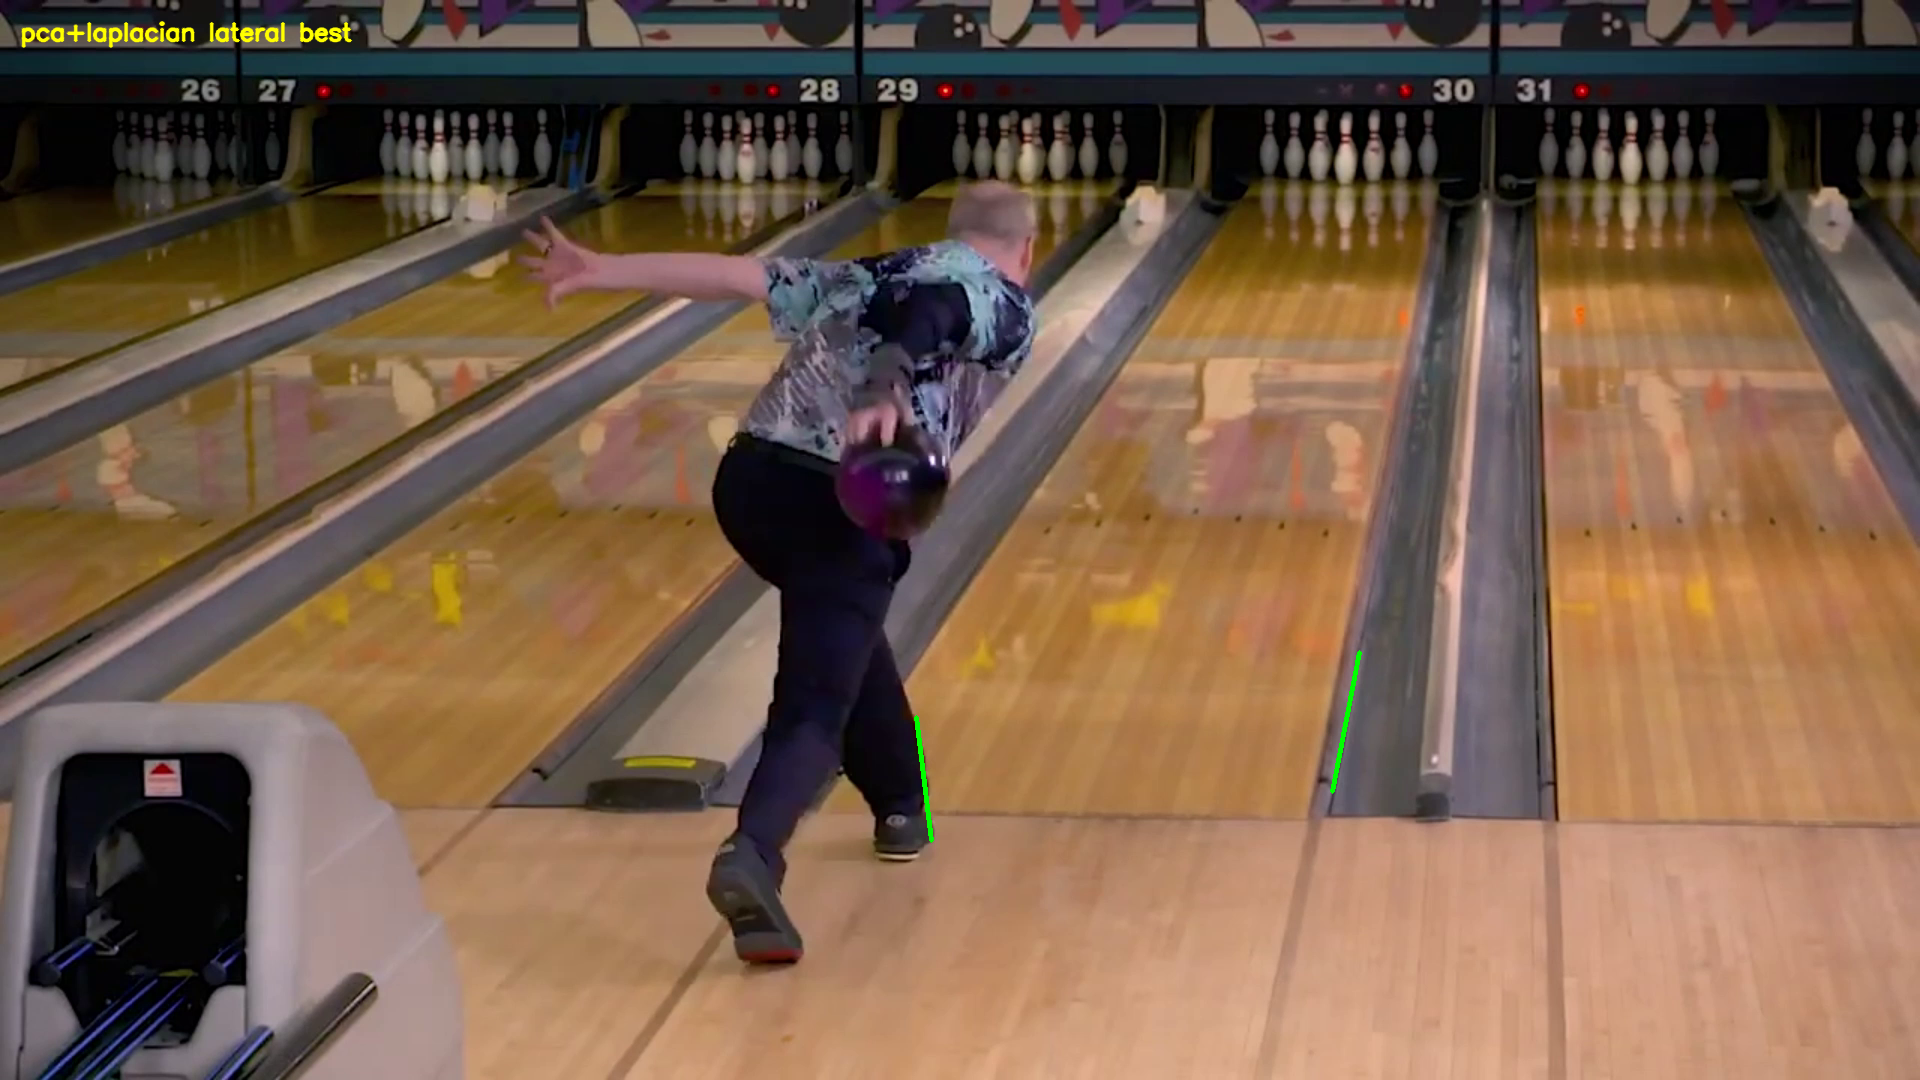
\includegraphics[width=0.48\textwidth]{figures/results/laplacian_over_sensitive.png}
    
    \vspace{0.2cm} % Adds a tiny bit of vertical breathing room between the rows
    
    % Bottom Row: The resulting bad quadrilaterals
    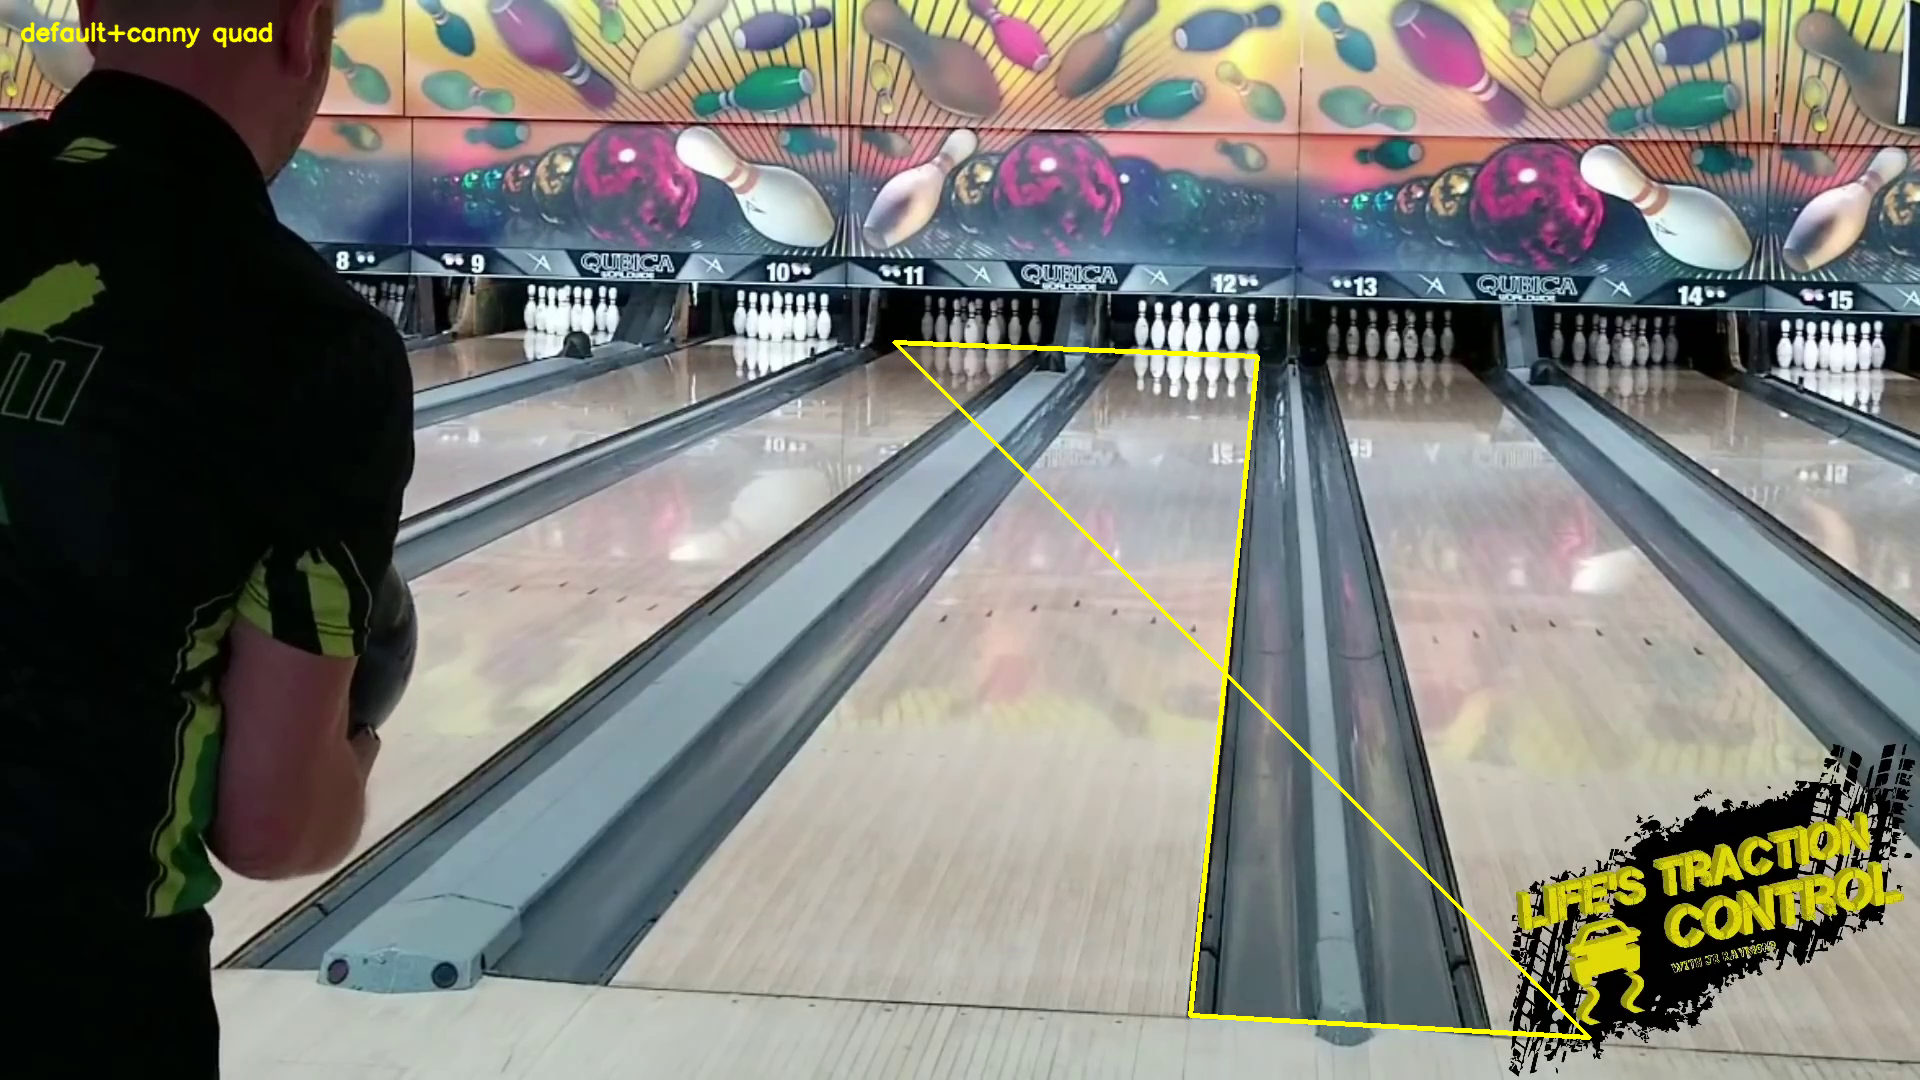
\includegraphics[width=0.48\textwidth]{figures/results/canny_over_sensitive_lane.png}
    \hfill
    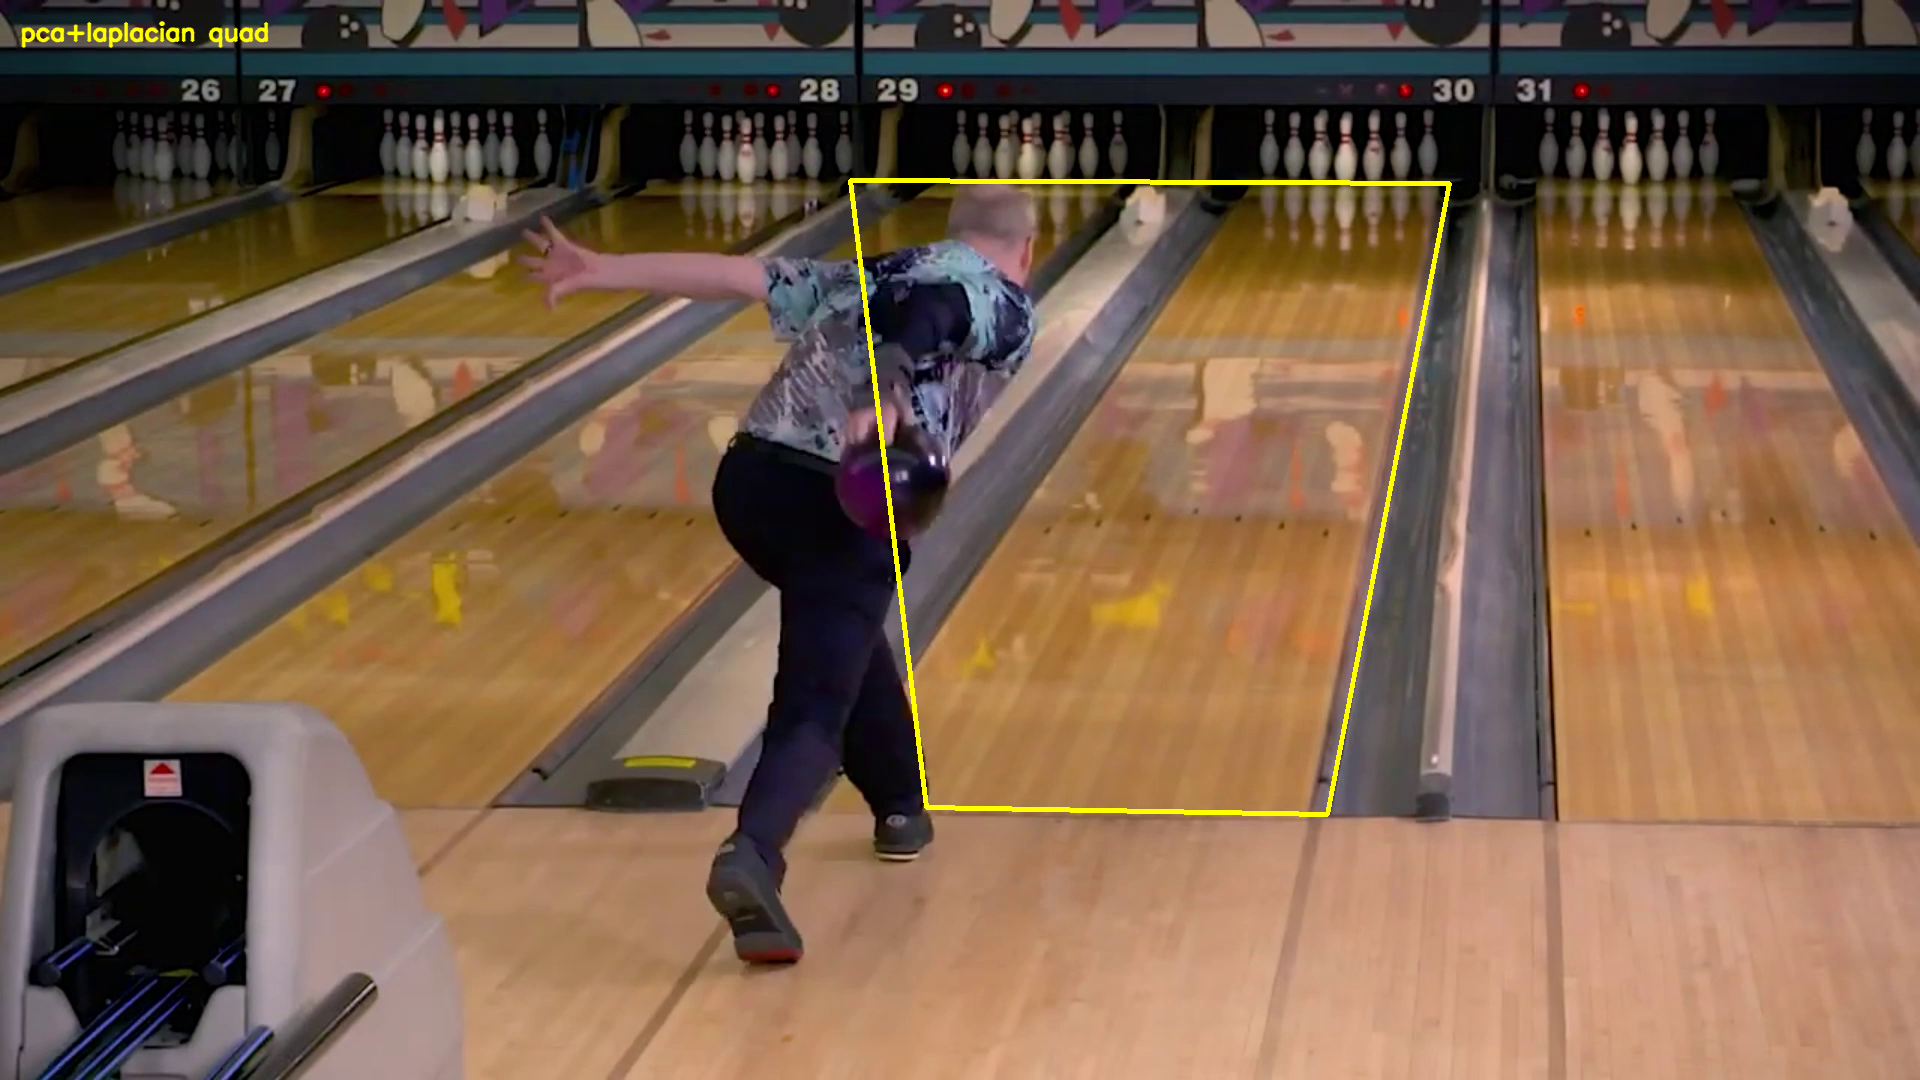
\includegraphics[width=0.48\textwidth]{figures/results/laplacian_over_sensitive_lane.png}
    
    \caption{Examples of heuristic failure due to over-sensitive edge detection. Top Left: Canny detects background wall structures. Top Right: Laplacian detects the bowler's leg and adjacent lane. Bottom Row: The respective incorrect homography quadrilaterals resulting from these flawed edge maps.}
    \label{fig:over_sensitive_edges}
\end{figure}

When evaluating single-channel color transformations, PCA proved superior in both general robustness and peak performance. Unlike fixed-weight channel conversions, PCA dynamically projects color channels onto their first principal component to maximize the statistical variance of each image. This data-driven approach adapts effectively to the highly variable wood types, oil patterns, and lighting found in bowling alleys. By isolating dominant structural features (the lane boards) while suppressing localized lighting artifacts, PCA achieved the highest stability across all edge detectors. When paired with the directionally targeted Sobel operator, the pipeline reached its peak performance, successfully extracting accurate lane boundaries in 7 out of 9 video clips. Consequently, the PCA and Sobel combination was selected for the final boundary detection module.

Finally, the analysis provided valuable insights into the theoretical limitations of chromatic edge detection. It was initially hypothesized that the Hue channel from the HSV color space might yield interesting results by isolating pure color transitions and entirely negating the impact of absolute brightness and shadows. In practice, however, the Hue channel demonstrated the poorest performance of the study, completely failing to localize boundaries across almost all filters. Qualitative analysis of the output (see Figure \ref{fig:hue_failure}) revealed the cause of this failure: the Hue representation effectively erased the critical geometric boundaries (particularly the bottom foul line) from the image entirely. This occurs because the physical demarcations of a bowling lane (such as a dark foul line or shaded gutters contrasting against the light wooden surface) are primarily defined by sharp shifts in luminance and intensity, rather than distinct shifts in core color. By stripping away the intensity information, the Hue channel eliminates the necessary gradient contrast, causing the borders to blend indistinguishably into the background. This visual evidence conclusively confirms that robust boundary extraction in a bowling setting relies fundamentally on structural intensity rather than pure chromaticity.



\begin{figure}[htbp]
    \centering
    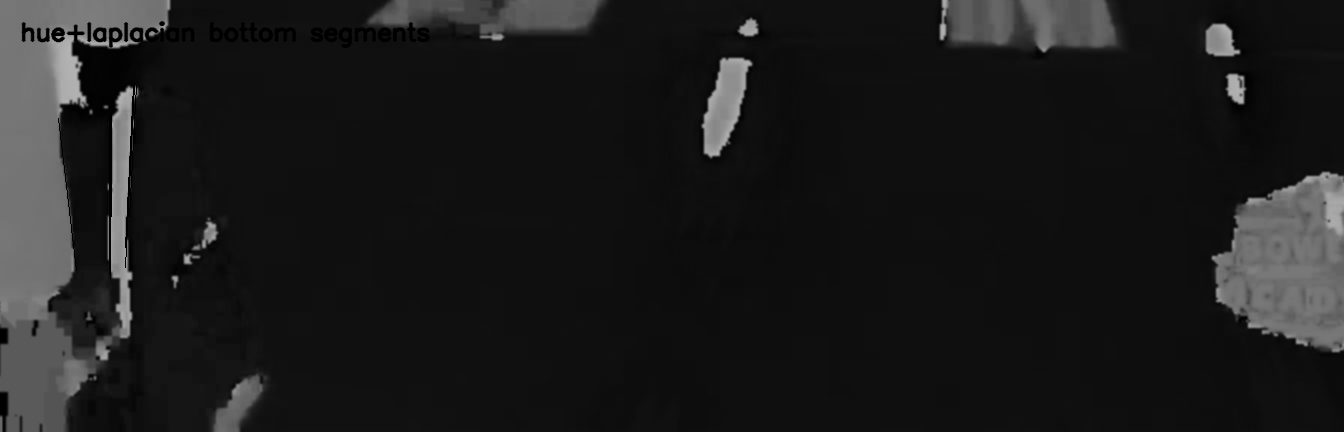
\includegraphics[width=0.6\textwidth]{figures/results/hue_removes_bottom_boundary.png}
    \caption{Output of the Hue channel on the lower lane segment. By discarding luminance data, the critical intensity contrast of the foul line is completely erased, resulting in a failure to detect the bottom boundary.}
    \label{fig:hue_failure}
\end{figure}
